\documentclass[
 reprint,
 amsmath,amssymb,
 aps,
]{revtex4-1}

\usepackage{graphicx}  
\usepackage{epstopdf}
\usepackage{dcolumn}
\usepackage{bm}	
\usepackage{amsmath}			
\usepackage{amsfonts}			
\usepackage{amssymb}			
\usepackage{latexsym}		
\usepackage{color}
\usepackage{ stmaryrd }
\begin{document}

\title{ 
Forward scattering of a plane wave and of a spatially smoothed laser pulse  in the hydrodynamic and kinetic frameworks }
\author{C. Ruyer}\email{charles.ruyer@cea.fr}
\affiliation{CEA, DAM, DIF, F-91297 Arpajon, France}
%\author{M. Grech}
%\affiliation{LULI - CNRS, CEA, UPMC Univ Paris 06: Sorbonne Universit\'e, Ecole Polytechnique, Institut Polytechnique de Paris - F-91128 Palaiseau Cedex, France}
\author{A. Debayle}
\affiliation{CEA, DAM, DIF, F-91297 Arpajon, France}
\author{P. Loiseau}
\affiliation{CEA, DAM, DIF, F-91297 Arpajon, France}
\author{M. Casanova}
\affiliation{CEA, DAM, DIF, F-91297 Arpajon, France}
\author{P. E. Masson-Laborde}
\affiliation{CEA, DAM, DIF, F-91297 Arpajon, France}

\begin{abstract}
We address the scattering of a high energy laser pulse on a   large wavelength acoustic turbulence of relevance for LMJ or NIF-class  experiments. 
Both kinetic and hydrodynamic framewaroks are adopted and combined with a linearized  description of the laser propagation. The resulting dispersion relations display important kinetic  contributions to the growth of the Forward Brillouin instability.  
Moreover, proof is made that the optical smoothing techniques  often used in high energy laser facilities are, for cold enough plasmas or in the multi ion species case, not enough to reach full control of the laser filamentation.
\textcolor{red}{Comparisons with experimental results, dedicated hydrodynamic and particle-in-cell simulations confirms our results. }
The   derived dispersion relations  present unique tools for assessing the propagation quality and energy deposition region of high energy lasers pulses. They also underlines the importance of accounting correctly for kinetic effects, even in the millimeters and nanoseconds scales of many  ICF or high-energy-density experiments. 
\end{abstract}

\maketitle

\section{Introduction}

%\begin{itemize}
   % \item It requires the precise predictions of the  laser propagation along with parametric instabilities and their coupling with the smoothing technics, routinely used in high energy class facilities \cite[]{NatPhys_Glenzer,NatPhys_Labaune}.  
    %\item Forward instabilities such as filamentation \cite[]{phd_Michel,POP_michel_2003,Lushnikov_2006,PRL_Sarri_2011}, forward Brillouin  or plasma smoothing effects \cite[]{phd-Grech,POP_Grech_2006,PRL_Grech_2009} are vastly unexplored, and let's be honest, far more complicated than playing ping pong with positrons.
%\end{itemize}
High energy class laser facilities such as LMJ,  NIF or ... routinely bring matter under extreme conditions, not only of interest for inertial confinement fusion \cite{Lindl_2004,SChina_Wang_2017,Cavailler_2005}, but also for high energy astrophysics \cite{Drake_2012} and high energy density physics   \cite{Drake2006}. 
Whether  the laser   serves as a heat source or as a diagnostics, the accurate prediction of its propagation remains crucial for designing and  conceive the experiment. Ergo, a large effort is made for understanding the wave mixing processes able to scatter a significant part of the electromagnetic energy in unwanted directions \cite[]{Shen_1965,Forslund_1973}. Stimulated backward Raman or Brillouin instabilities  \cite{POP_Liu_2009,hao_2013},  cross beam energy transfer \cite{hao_2016}  or collective scattering  \cite[]{PRL_Neuville_2016,PRL_Depierreux_2016} embody critical issues and active area of research.
Additionally, hydrodynamic codes, vastly used due to their relatively affordable numerical cost, either require \emph{ad hoc} corrections or otherwise simply  omit, kinetic-based processes such as the particle trapping and subsequent wave-breaking \cite[]{POP_Benisti_2008,POP_Berger_2013}, two plasmon decay \cite[]{Dubois_1995,Russell_2001} or non-local thermal diffusion \cite[]{POP_Schurtz_2000,PRL_Froula_2007}, affecting the associated laser energy deposition. 
In this context, a better control of the laser propagation could be achieved by the use of spectral dispersion (SSD) and  random phase plates (RPP) optical smoothing techniques  \cite[]{Kato_1984,NatPhys_Glenzer,NatPhys_Labaune}.  
However, the resulting micron-scale speckle dynamics  interweave with the wave mixing processes, bringing further complexity to the theoretical and numerical analysis \cite[]{POP_Duluc_2019}. 
Conspicuously, the filamentation instability \cite[]{phd_Michel,POP_michel_2003,Lushnikov_2006,PRL_Sarri_2011}, forward Brillouin  scattering or plasma smoothing effects \cite[]{phd-Grech,POP_Grech_2006,PRL_Grech_2009} 
are very challenging to properly encompass  in nanosecond and millimeter scale laser-plasma studies.

This publication ambitions are to convey new tools 
able to address  the spatial growth of an electromagnetic scattered wave of wavevector and frequency close to the PP pulse's and embed in driven acoustic density fluctuations.
We first derive both the kinetic and fluid forward scattering of a plane wave, \emph{i.e.} the  stimulated forward Brillouin scattering (FSBS) and the filamentation instabilities and pinpoints the importance of accounting for the kinetic plasma response for understanding quantitatively the scattering growth.
From  a simple model of Random Phase Plate smoothed laser beam ensues our RPP dispersion relations  able to predict the growth of the forward scatter relevant for high energy laser experiments. 
\textcolor{red}{Dedicated "particle-in-cell" (PIC) simulations allows to validate our predictions and underline the importance of accounting for the laser smoothing in order to understand the forward Brillouin growth. 
Moreover, a comparison with an hydrodynamic simulation and a RPP filamentation experiment conducted at the LULI facility confirms the relevance of our calculation concerning realistic plasma conditions.} 
The last section gather our perspective and concluding remarks. 

Finally, the SI unit system is used throughout this study and vectors are noted in bold symbols. 

\section{Spatial growth of the  forward scattering of a plane wave}\label{sec:plane}
\subsection{Fluid and kinetic general dispersion relation}
The simplest way to obtain the growth of the forward scattering of a light wave propagating in a plasma consists  in combining the perturbed Maxwell equations with a linearized plasma response, either kinetic or fluid.
We aim at deriving and comparing in this section both frameworks.

Following Refs. \cite[]{Kruer,phd_Michel}, the perturbation of Maxwell equations around the laser fields, $E_0$, \emph{i.e.} $E = E_0 + \delta E$ and around the  electron density at rest $n_e = n_{e0}+\delta n_e$, gives in the Fourier space $(\omega_d,\mathbf{k}_d)$
\begin{equation}
    (\omega_d^2 - \omega_{pe}^2 -\mathbf{k}_d^2c^2)\delta E(\omega_d,\mathbf{k}_d) = \omega_0^2 \frac{\delta n_e }{n_c}\otimes E_0  \, ,\label{eq:max1}
\end{equation}
where $\omega_{pe}$, $\omega_{0}$,  $n_c$ and $c$ are the plasma and laser frequency, laser critical density and light speed in vacuum respectively. Use has also been made of $\otimes$ which designates  here a convolution product in the Fourier space.
Introducing a space and time envelop in the vicinity of the laser field, $E_0\equiv E_0 \cos(k_0 x - \omega_0t)$,
we may write in the Fourier space,  $E_0 =[ \delta(\omega-\omega_0, \mathbf{k}-\mathbf{k}_0) + \delta(\omega+\omega_0, \mathbf{k}+\mathbf{k}_0) ]E_0/2 $, which yields 
\begin{align}
    (\omega_d^2 - \omega_{pe}^2 -\mathbf{k}_d^2c^2)\delta E(\omega_d,\mathbf{k}_d) = \frac{\omega_0^2}{2} E_0\times \nonumber\\ \left[\frac{\delta n_e }{n_c}(\omega_d-\omega_0, \mathbf{k}_d-\mathbf{k}_0) +\frac{\delta n_e }{n_c}(\omega_d+\omega_0, \mathbf{k}_d+\mathbf{k}_0) \right] \, ,\label{eq:max2}
\end{align}

The final dispersion relation  can be obtained by combining this equation with a linearized plasma response, which in the fluid framework for a plasma at rest %($v_d=0$) 
reads 
\begin{align}
   \frac{\delta n_e }{n_{e0}}(\omega_s,\mathbf{k}_s) = \frac{-\mathbf{k}^2c_s^2}{ \mathbf{k}_s^2c_s^2-\omega_s^2 -2i\omega_s \nu} \frac{A_k\epsilon_0 E_0}{n_c T_e}\times \nonumber\\ \left[\delta E(\omega_s-\omega_0, \mathbf{k}_s-\mathbf{k}_0) +\delta E(\omega_s+\omega_0, \mathbf{k}_s+\mathbf{k}_0) \right] \, ,\label{eq:fluid}
\end{align}
where $c_s\simeq [(Z_iT_e+3 T_i)/m_i]^{1/2}$, $\nu=\vert\mathbf{k}_s\vert \gamma_0 c_s$ and $A_k$ are respectively  the sound speed, Landau damping frequency and non-local correction to the ponderomotive force  as introduced in Ref. \cite[]{Bychenkov_2000}, 
\begin{align}
     A_k(u)   &= \frac{1}{2} +Z\left( \frac{0.074}{u^2}+ \frac{0.88}{u^{4/7}} + \frac{2.54}{1+5.5u^2} \right) \, ,\nonumber \\ 
     u &=\vert \mathbf{k}_s \vert\lambda_\mathrm{mfp} \sqrt{Z_i}\label{eq:nl}\, .
\end{align}
We also made use of $T_{e/i}$, $m_{e/i}$ $Z_i$ and $\lambda_\mathrm{mfp}$ the electron/ion temperature and mass, ion charge number and electron mean-free-path.

Likewise, the kinetic counterpart of Eq. \eqref{eq:fluid} has been derived in Ref. \cite[]{POF_Drake_1973} and    takes on, for a multiple ion plasma, 
\begin{align}
 \frac{ \delta n (\omega_s, \mathbf{k}_s ) }{n_{e0}}  =   \frac{ \epsilon_0  E_0 }{ 2n_c T_e } 
 \frac{\mathcal{Z}'( \xi_e) }{2}
 \frac{\sum_i\mathcal{Z}'( \xi_i)\frac{  Z_iT_e}{ T_i }\frac{  Z_in_i}{ n_e }   }{  \mathcal{Z}'( \xi_e)+ \sum_i\mathcal{Z}'( \xi_i)\frac{  Z_iT_e}{ T_i }\frac{ Z_i n_i}{ n_e }  }
 % \frac{\mathcal{Z}'( \xi_i)   }{  \mathcal{Z}'( \xi_i) +\mathcal{Z}'( \xi_e)\frac{ T_i }{  ZT_e} }
\nonumber\\  \times \left[\delta E(\omega_s-\omega_0, \mathbf{k}_s-\mathbf{k}_0) +\delta E(\omega_s+\omega_0, \mathbf{k}_s+\mathbf{k}_0) \right] %\nonumber \\  &\times 
   \, ,\label{eq:drake}\\
   \xi_{e/i} = \frac{   \omega }{   \vert\mathbf{k}_s\vert }  \sqrt{ \frac{ m_{e/i } }{ 2T_{e/i }}  }  \label{eq:xi} \, , 
 \end{align}
 where, for an ion Debye length $\lambda_{Di}$, we assumed $\vert k_s \lambda_{Di} \vert \ll 1$. 
We introduced $\mathcal{Z}$, the plasma dispersion function \cite{Fried_Gell-Mann_1960} and its arguments $\xi_{e } $ and $\xi_{i }$. %, which in turn depend on $\mathbf{v}_d$, the electron/ion   drift velocity.

In order to be combined with Eq. \eqref{eq:max2}, we may recast, for $v_\phi = \omega_s/\vert \mathbf{k}_s\vert $, Eqs. \eqref{eq:fluid} and  \eqref{eq:drake} into 
\begin{align}
   \frac{\delta n_e }{n_{e0}}(\omega_s,\mathbf{k}_s) = -\alpha_{k/f}(v_\phi) \frac{A_k\epsilon_0 E_0}{n_c T_e}\times \nonumber\\ \left[\delta E(\omega_s-\omega_0, \mathbf{k}_s-\mathbf{k}_0) +\delta E(\omega_s+\omega_0, \mathbf{k}_s+\mathbf{k}_0) \right] \, ,\label{eq:fd} \\
   \alpha_k  = \frac{\mathcal{Z}'( \xi_e) }{2}\frac{\mathcal{Z}'( \xi_i)   }{  \mathcal{Z}'( \xi_i) +\mathcal{Z}'( \xi_e)\frac{ T_i }{  ZT_e} }\, ,\label{eq:alphak} \\
   \alpha_f = \frac{c_s^2}{ c_s^2-v_\phi^2 -2iv_\phi c_s \gamma_0}\, .\label{eq:alphaf}
\end{align}
Note that we have  applied the so-called non-local correction [Eq. \eqref{eq:nl}] in the kinetic framework, as there is, to the best of our knowledge,  no counter-argument for doing so. 

From the combination of  Eqs. \eqref{eq:max2} with \eqref{eq:fd}, 
for $D_\pm= (\omega_s-\omega_0)^2 - \omega_{pe}^2 -( \mathbf{k}_s-\mathbf{k}_0) ^2c^2 $, ensues
\begin{equation}\label{eq:dispe}
    D_+D_- = -\frac{\omega_{0}^2}{2}\alpha_{k/f}A_k\frac{\delta n_0}{n_c} (D_++D_-) \, ,
\end{equation}
with $\delta n_0/n_c = (n_{e0}/n_c) \epsilon_0E_0^2/(n_c T_e)$.
Note that we neglected the terms in $\delta n_e(\omega_s \pm 2\omega_0)$.
In the kinetic framework, the above equation corresponds to Eq. (36) of Ref. \cite[]{POF_Cohen_79} in the limit $\vert k_s \lambda_{Di} \vert \ll 1$. In the fluid framework, these equations were derived in Refs. \cite[]{Kruer,phd_Michel,phd-Grech} \textcolor{red}{(?)}.

\subsection{Spatial growth of the filamentation and of the forward Brillouin instability}
Hence,  making use of $\omega_0^2=\omega_{pe}^2 +k_0^2c^2$, we may simplify $D_\pm$ to leading order in $\omega_s\ll\omega_0$, giving 
\begin{equation}\label{eq:dpm}
D_\pm = -\mathbf{k}_s^2c^2\pm 2(\omega_s\omega_0 - \mathbf{k}_s\cdot\mathbf{k}_0 c^2) \, .
\end{equation} 
Equation \eqref{eq:dispe} thus becomes 
\begin{equation}\label{eq:dispe2} 
(\omega_s\omega_0 - \mathbf{k}_s\cdot\mathbf{k}_0 c^2)^2
=\frac{\mathbf{k}_s^2c^2}{4}\left( \mathbf{k}_s^2c^2 - \omega_{0}^2\alpha_{k/f}(v_\phi)A_k\frac{\delta n_0}{n_c} \right) 
\, .
\end{equation}

The spatial growth of the filamentation instability may be recovered when $\omega_s$=0 and assuming a $\mathbf{k}_s = k_s \hat{\mathbf{x}} +i\Gamma_F \hat{\mathbf{y}}$ ($\hat{\mathbf{x}}=\mathbf{k}_0 /\vert \mathbf{k}_0 \vert $ and  $\hat{\mathbf{y}}$  are unity vectors in the $x$ and $y$ directions respectively), and 
\begin{equation}\label{eq:gf} 
\Gamma_F^2
=\frac{\mathbf{k}_s^2c^2}{4}\left( \omega_{0}^2\alpha_{k/f}(0)A_k\frac{\delta n_0}{n_c}- \mathbf{k}_s^2c^2 \right) 
\, .
\end{equation}
Note that $\alpha_f(0)=1$ and $\alpha_k(0)=\sum_i Z_iT_e/T_i/(1+\sum_i Z_iT_e/T_i)$ so that the kinetic and fluid frameworks con\"incide in the limit $Z_iT_e/T_i\gg 1$ for at least one ion species.

As for the forward Brillouin scattering,  corresponding to the limit $1/D_-\gg1/D_+$, non vanishing acoustic wave frequencies are obtained with  phase speeds of the order of the sound speed. We propose to address the spatial growth of both the filamentation and forward Brillouin instability  by solving Eq. \eqref{eq:dispe2} for  $\mathbf{k}_s = k_{sx} \hat{\mathbf{x}} +k_{sy} \hat{\mathbf{y}}$, and assuming 
$ k_{sy}$ and $k_{sx}$ complex and purely real   respectively. Equation \eqref{eq:dispe2} then becomes 
\begin{equation}\label{eq:dispe3} 
\left(\frac{v_\phi}{\eta c} - 
\frac{ k_{sx}}{\vert \mathbf{k}_s\vert }\right)^2
=\frac{1}{4} \left( \frac{\mathbf{k}_s^2}{k_0^2} - \alpha_{k/f}(v_\phi)A_k\frac{\delta n_0}{\eta^2n_c} \right) 
\, ,
\end{equation}
where $\eta=\sqrt{1-n_{e0}/n_c}$ is the refraction index.
Hence, $u =  k_{sx}/\vert \mathbf{k}_s\vert $ is solution of the following second order polynomial equation, 
\begin{equation}\label{eq:dispe2poly} 
u^2 -2\frac{v_\phi}{\eta c}u +\frac{v_\phi^2}{\eta^2 c^2}-\frac{1}{4}\left( \frac{\mathbf{k}_s^2}{k_0^2} - \alpha_{k/f}(v_\phi)A_k\frac{\delta n_0}{\eta^2n_c} \right) =0 
\, .
\end{equation}
To leading order in  $\Im(k_{sx})/\vert \mathbf{k}_s\vert $ (where $\Im$ and $\Re$ are the imaginary and real part of a complex), $\vert \mathbf{k}_s\vert$ and $v_\phi$ may be considered to be purely real.

\begin{figure}
\begin{tabular}{cc}
(a) Kinetic, $\Gamma/k_0$ &
(b)  Kinetic, $\Re(k_{sx})$ \\
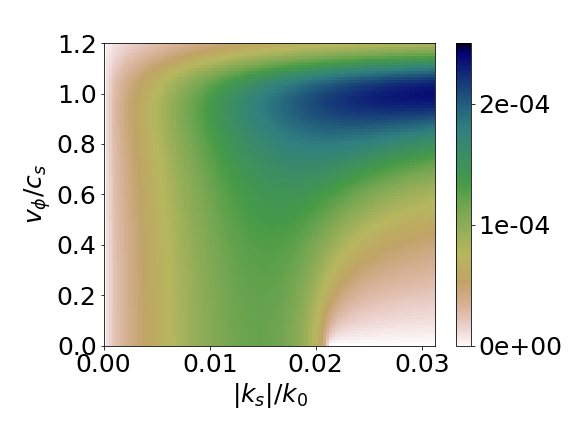
\includegraphics[width=0.24\textwidth]{G_Te1keV_Ti300_3e14_3w_1e-1nc_Hp.png}&
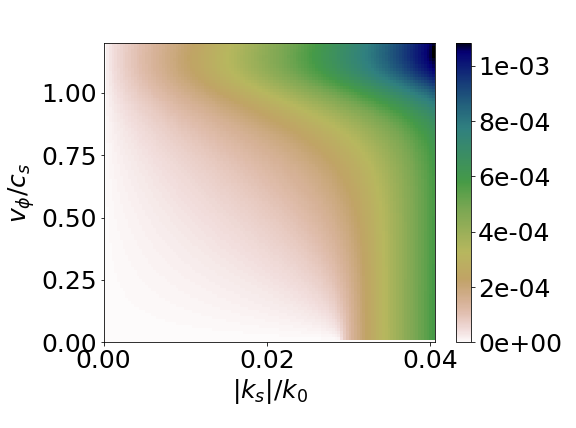
\includegraphics[width=0.24\textwidth]{k_Te1keV_Ti300_3e14_3w_1e-1nc_Hp.png}\\
(c) Fluid, $\Gamma/k_0$  &
(d) Fluid, $\Re(k_{sx}/k_0)$  \\
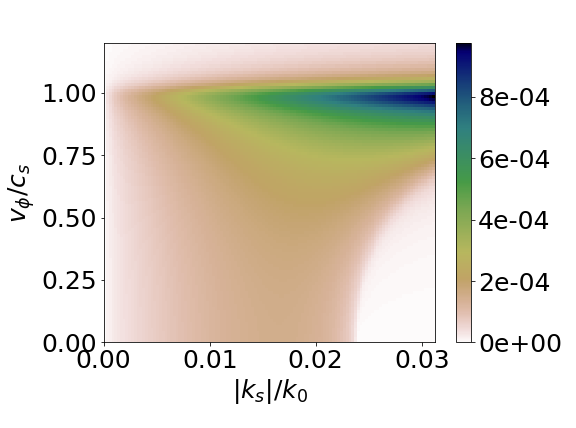
\includegraphics[width=0.24\textwidth]{Gf_Te1keV_Ti300_3e14_3w_1e-1nc_Hp.png}&
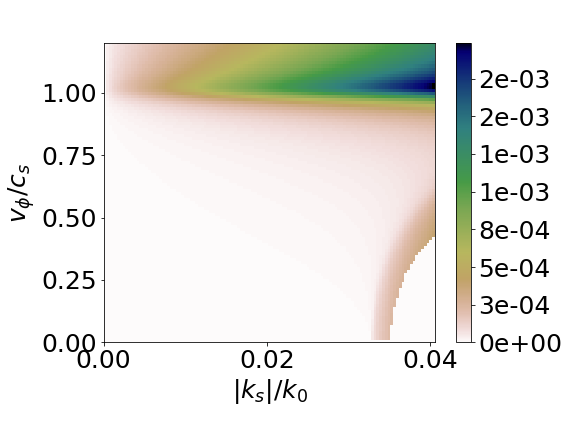
\includegraphics[width=0.24\textwidth]{kf_Te1keV_Ti300_3e14_3w_1e-1nc_Hp.png}
\end{tabular}
\caption{ \label{fig:dispe}  
Kinetic (a,b) and fluid (c,d) resolution of Eq. \eqref{eq:dispe2poly} for  $I_0 = 3\cdot 10^{14}\, \rm W.cm^{-2}$, $2\pi/k_0=0.35 \,\rm\mu m$, $T_e =1\,\rm  keV$, $ T_i=300\,  \rm eV$ in a H$^+$ and $n_{e0}=0.1n_c$.
 }
\end{figure}
\begin{figure}
\begin{tabular}{cc}
(a) Kinetic, $\Gamma/k_0$ &
(b)  Kinetic, $\Re(k_{sx})$ \\
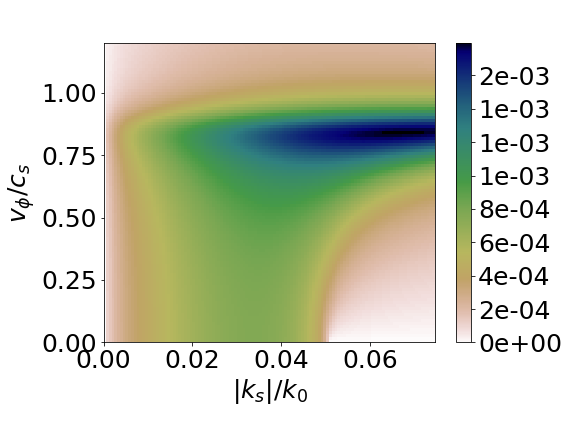
\includegraphics[width=0.24\textwidth]{G_Te700eV_Ti500_3e14_3w_1e-1nc_CH.png}&
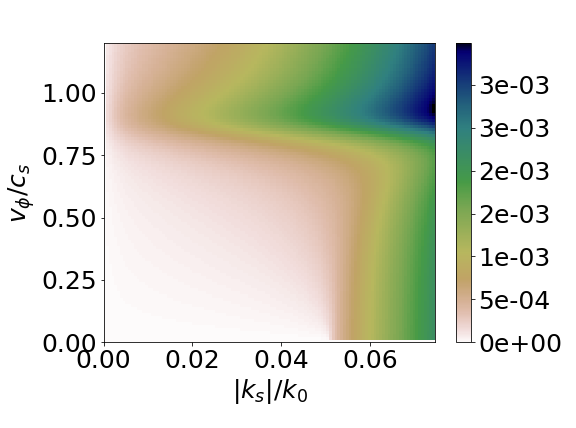
\includegraphics[width=0.24\textwidth]{k_Te700eV_Ti500_3e14_3w_1e-1nc_CH.png}\\
(c) Fluid, $\Gamma/k_0$  &
(d) Fluid, $\Re(k_{sx}/k_0)$  \\
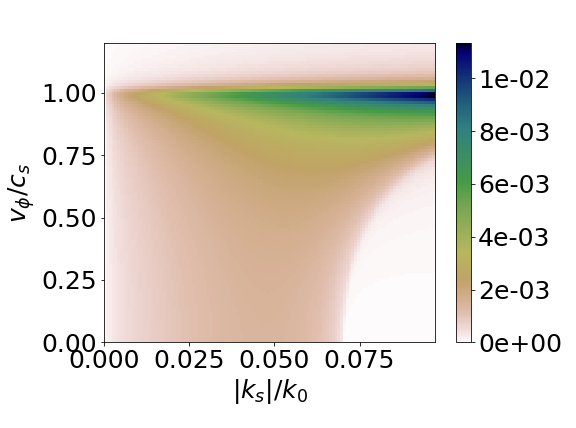
\includegraphics[width=0.24\textwidth]{Gf_Te700eV_Ti500_3e14_3w_1e-1nc_CH.png}&
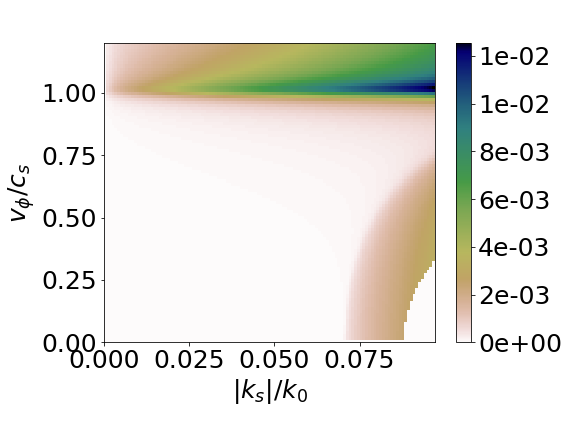
\includegraphics[width=0.24\textwidth]{kf_Te700eV_Ti500_3e14_3w_1e-1nc_CH.png}
\end{tabular}
\caption{ \label{fig:dispeCH}  
Kinetic (a,b) and fluid (c,d) resolution of Eq. \eqref{eq:dispe2poly} for  $I_0 = 3\cdot 10^{14}\, \rm W.cm^{-2}$, $2\pi/k_0=0.35 \,\rm\mu m$, for a CH plasma with $n_c=n_H$, $T_e =700\,\rm  eV$, $T_C=T_H =500\,  \rm eV$ and $n_{e0}=0.1n_c$. The value of the non-local correction [Eq. \eqref{eq:nl}], is obtained with the carbon parameters, corresponding to the smallest electron-ion mean-free-path. Use is made of the mean charge number, mean mass number   for calculating the sound speed and normalized Landau damping rate $c_s$ and $\gamma_0$.
 }
\end{figure}
Figures \ref{fig:dispe}(a-d) displays  $\Re(k_{sx})$ and the spatial growth rate,  $\Gamma=-\Im(k_{sx})$, solution of Eq. \eqref{eq:dispe2poly} as a function of the phase speed and of the wavevector amplitude, in both the kinetic (a,b) and fluid framework (c,d). The filamentation limit is recovered at $v_\phi=0$ and care has been taken to verify that, when $T_i\ll Z_iT_e$, both frameworks con\"incide. Moreover, in both calculations, $\Re[k_{sx}(v_\phi=0)]$ is vanishing as expected from the filamentation instability. As $v_\phi$ increases, one starts to enter in the forward Brillouin instability domain which peaks, for the kinetic  mono-ion species case of Fig. \ref{fig:dispe}(a), around $(\vert k_s\vert/k_0, v_\phi/c_s) \simeq(0.03,1)$. Interestingly, only in the kinetic framework  the forward Brillouin spatial maximum  growth dominates the filamentation one. In the fluid framework however both instability present a close  growth rate of $\sim 1.5\times 10^{-4} k_0$  with much  broader  spectrum than in the kinetic case.

The kinetic calculations allow to consider multiple ion plasmas such as CH  illustrated in Fig. \ref{fig:dispeCH}. In the fluid framework, we are usually constrained to use the averaged-ion approximation, which gives qualitatively similar results than for Fig. \ref{fig:dispe}(c) as a broad spectrum is evidenced with no dominance of Brillouin versus filamentation. 

For both Figs. \ref{fig:dispe} and \ref{fig:dispeCH},   from the kinetic framework ensues a  roughly twice lager maximum forward Brillouin growth rate than in the fluid framework,  and comparable results are obtained regarding the filamentation instability. 
The growth of propagating ($\vert v_\phi\vert >0$) ion acoustic wave   is able to the scattered the pump wave and modify its spatial spectrum. As evidenced in Fig. \ref{fig:dispe}(a,d) and \ref{fig:dispeCH}(a,d) we expect a broadening of the plane wave spatial spectrum  resulting in an f-cone   of angle $k_s/k_0\sim 0.03-0.05$, corresponding to $\sim 2-3^o$.  

The spatial (RPP) or temporal (SSD) of energetic laser pulses is commonly known to restrain the role of deleterious instabilities, such as the laser filamentation, on the propagation of the beam \cite[]{Kato_1984,NatPhys_Glenzer}. Indeed, as shown in this section, the most unstable wavelength, regarding the filamentation or the forward Brillouin instabilities, is of the order of ten   microns (for $\sim$ keV and 10\% critical density plasmas), thus smaller than the typical  speckle size   of a few microns   usually used in energetic laser facilities.  
Hence, the plane wave approximation used in obtaining Eq. \eqref{eq:max2} no longer holds and one expects a more stable pump propagation.
Although, extensively studied in the fluid framework by mean of simulation tools \cite[]{}, to the best of our knowledge, no analytical attempts were made to estimate the spatial growth of the forward Brillouin scattering of an RPP pulse, especially in the kinetic framework. 
We propose in next section to adapt the above analytical plane wave dispersion relations  to the propagation of energetic RPP pulse.

 \begin{widetext}
\section{Forward scattering of a spatially smoothed laser pulse}
\subsection{Kinetic and fluid dispersion relations}
The  beam model adopted here has been introduced in  Refs. \cite[]{POF_Schmitt_88,POF_Rose_93} and presents an electric field which follows at the focal plane,
 \begin{align}
E_0(t,\mathbf{r})  = \frac{E_0}{N} \sum_{n,\vert k_{\perp}\vert<k_m }^N  \cos(k_0x - \omega_0t +\mathbf{k}_\perp(n) \cdot \mathbf{r}_\perp +\Phi_{\mathbf{k}_\perp})\, , \label{eq:erpp}
 \end{align}
 where  $N$ is the number of diffracting elements and the phases $\Phi_{\mathbf{k}_\perp}$ are  independent random variables taking the values $0$ or $\pi$ with equal probability.
 For simplicity, we will assume a square phase plate that verifies $k_{\perp}(n) = n2k_m/N$ and  $n$ an integer with $n\in \llbracket - N/2 ,N/2 \rrbracket$ and $k_m = k_0/(2f_\sharp)$. 
 Under these conditions, and for $\langle w\rangle$ representing the statistical average of $w$,  we note   that,
 \begin{equation}\label{eq:d}
 \langle e^{i\Phi_{k_1}+i\Phi_{k_2}}\rangle=\delta(k_1-k_2) \, .
 \end{equation}

We will now follow the procedure introduced in Sec. \ref{sec:plane} while replacing the plane pump wave by the fields given by Eq. \eqref{eq:erpp}. Hence, we will start by writing the RPP electric field in Fourier space and enveloped around the laser frequency and wavevectors $\omega_0$ and $k_0$,
\begin{align}
E_0(\omega,\mathbf{k}) = \frac{E_0}{2N} \sum_{\ k_{\perp} }[ e^{i\Phi_{k_\perp}}\delta(\omega-\omega_0, \mathbf{k}-\mathbf{k}_\perp)    + e^{-i\Phi_{k_\perp}}\delta(\omega+\omega_0, \mathbf{k}+\mathbf{k}_\perp) ]
\, , \label{eq:erppf}
\end{align}
 where $\mathbf{k}_\perp= k_0\hat{\mathbf{x}} +k_\perp \hat{\mathbf{y}}$ and the sum runs over $k_\perp$ for $\vert k_\perp\vert  <k_m$.
 Combined with the perturbed Maxwell equations [Eq. \eqref{eq:max1}], we obtain
 \begin{align}
    (\omega_d^2 - \omega_{pe}^2 -\mathbf{k}_d^2c^2)\delta E(\omega_d,\mathbf{k}_d) = \frac{\omega_0^2}{2N} E_0 \sum_{\ k_{\perp} }   \left[e^{i\Phi_{k_\perp}}\frac{\delta n_e }{n_c}(\omega_d-\omega_0, \mathbf{k}_d-\mathbf{k}_\perp) +e^{-i\Phi_{k_\perp}}\frac{\delta n_e }{n_c}(\omega_d+\omega_0, \mathbf{k}_d+\mathbf{k}_\perp) \right] \, .\label{eq:maxrpp}
\end{align}
Likewise, the plasma linear response, either kinetic or fluid, involves a convolution product between $E_0(\omega_0,\mathbf{k}_\perp)$ and $\delta E(\omega_d,\mathbf{k}_d)$ which yields,
\begin{align}
   \frac{\delta n_e }{n_{e0}}(\omega_s,\mathbf{k}_s) = -\alpha_{k/f}(v_\phi) \frac{A_k\epsilon_0 E_0}{Nn_c T_e} \sum_{\ k_{\perp} }     \left[e^{i\Phi_{k_\perp}}\delta E(\omega_s-\omega_0, \mathbf{k}_s-\mathbf{k}_{\perp}) +e^{-i\Phi_{k_\perp}}\delta E(\omega_s+\omega_0, \mathbf{k}_s+\mathbf{k}_{\perp}) \right] \, ,\label{eq:fdrpp} 
\end{align}
When plugging Eq. \eqref{eq:maxrpp} into \eqref{eq:fdrpp}, two sums will appear, noted with two independent index, $k_1$ and $k_2$. Hence, as for the derivation of Eq. \eqref{eq:dispe}, we will neglect the terms in $\delta n_e(\omega_s\pm 2\omega_0)$ that are considered too far from resonance. With $D_\pm(k_{1})= (\omega_s-\omega_0)^2 - \omega_{pe}^2 -( k_{sx}-k_0) ^2c^2 -( k_{sy}-k_{1}) ^2c^2$ and $\mathbf{k}_{1,2}= k_0\hat{\mathbf{x}} +k_{1,2} \hat{\mathbf{y}}$, we obtain
\begin{align}
   \frac{\delta n_e }{n_{e0}}(\omega_s,\mathbf{k}_s) = -\alpha_{k/f}(v_\phi)A_k \frac{\delta n_0}{n_c} \frac{\omega_0^2}{2N^2}\sum_{ k_{1} } \sum_{ k_{2} }        \left[ \frac{e^{i\Phi_{k_1}-i\Phi_{k_2}} }{D_-(k_{1})}\frac{\delta n_e }{n_{e0}}(\omega_s,\mathbf{k}_s-\mathbf{k}_{1}+\mathbf{k}_{2}) +\frac{e^{-i\Phi_{k_1}+i\Phi_{k_2}}}{D_+(k_{1})} \frac{\delta n_e }{n_{e0}}(\omega_s,\mathbf{k}_s+\mathbf{k}_{1}-\mathbf{k}_{2}) \right] \, ,\label{eq:fddrpp} 
\end{align}
 \end{widetext}
 
 \begin{figure}
\begin{tabular}{cc}
(a) Kinetic, $\Gamma/k_0$ &
(b)  Kinetic, $\Re(k_{sx})$ \\
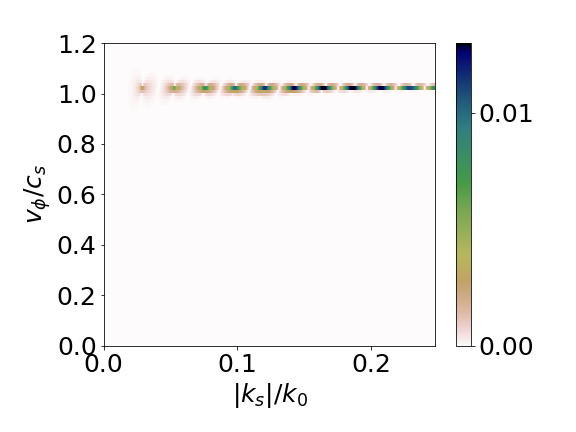
\includegraphics[width=0.25\textwidth]{Grpp_Hp.png}&
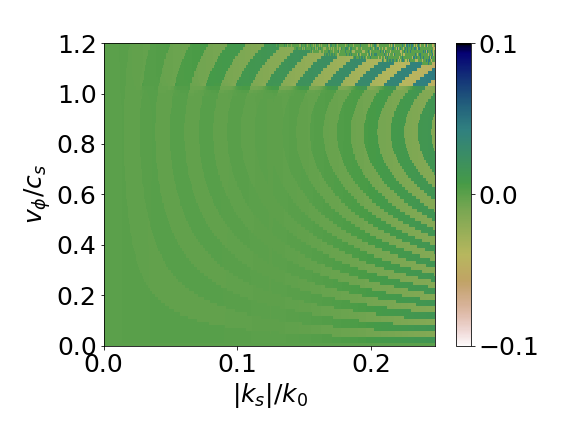
\includegraphics[width=0.25\textwidth]{krpp_Hp.png}\\
(c) Fluid, $\Gamma/k_0$  &
(d) Fluid, $\Re(k_{sx}/k_0)$  \\
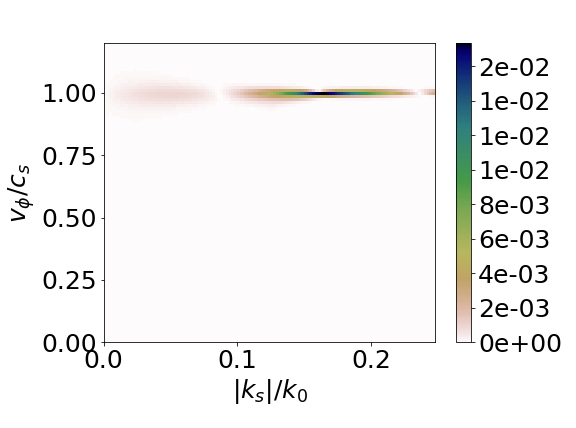
\includegraphics[width=0.25\textwidth]{Gfrpp_Hp.png}&
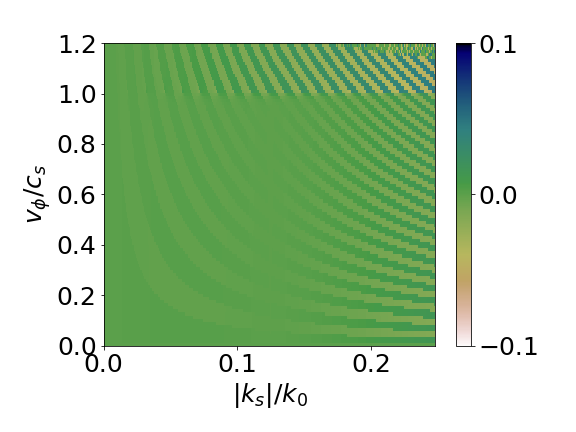
\includegraphics[width=0.25\textwidth]{kfrpp_Hp.png}
\end{tabular}
\caption{ \label{fig:disperpp}  
Kinetic (a,b) and fluid (c,d) resolution of Eq. \eqref{eq:dispe2polyrpp} for  the same parameters than in Fig. \ref{fig:dispe} but with an RPP beam given by Eq. \eqref{eq:erpp} with $f_\sharp=8$. 
 }
\end{figure}
\begin{figure}
\begin{tabular}{cc}
(a) Kinetic, $\Gamma/k_0$ &
(b)  Kinetic, $\Re(k_{sx})$ \\
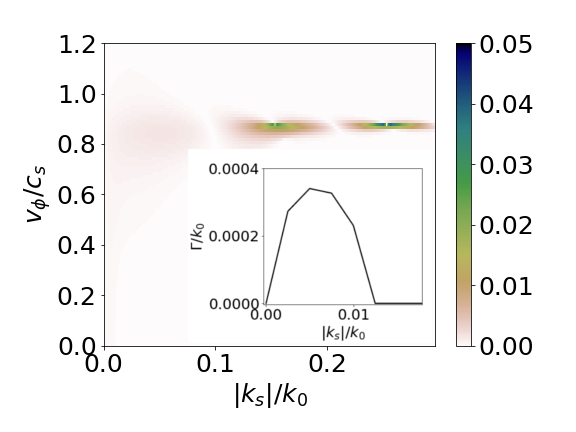
\includegraphics[width=0.24\textwidth]{Grpp_CH_new.png}&
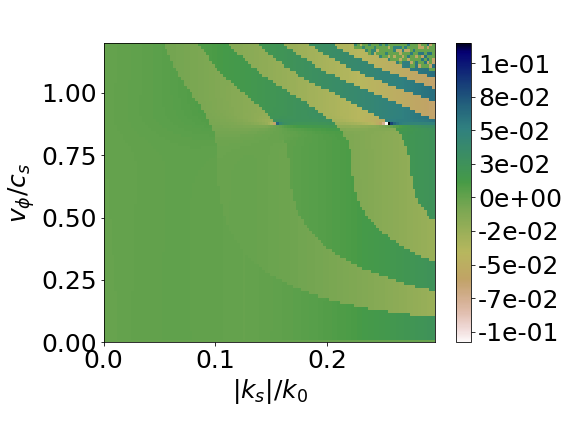
\includegraphics[width=0.24\textwidth]{krpp_CH.png}\\
(c) Fluid, $\Gamma/k_0$  &
(d) Fluid, $\Re(k_{sx}/k_0)$  \\
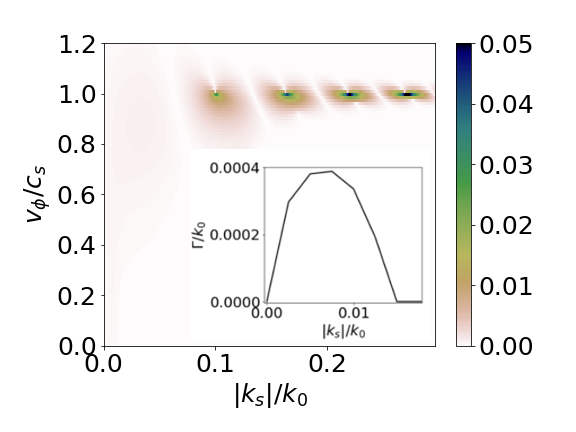
\includegraphics[width=0.24\textwidth]{Gfrpp_CH_new.png}&
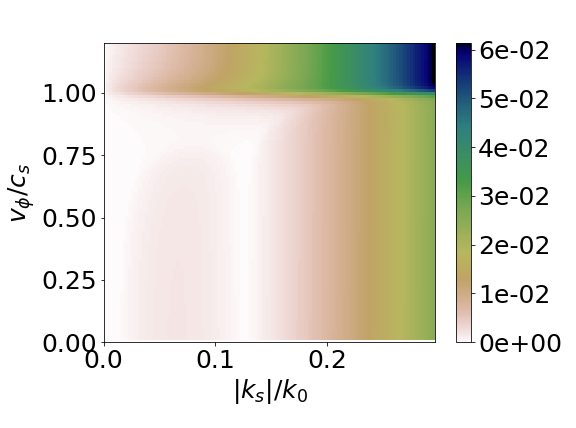
\includegraphics[width=0.24\textwidth]{kfrpp_CH.png}
\end{tabular}
\caption{ \label{fig:dispeCHrpp}  
Kinetic (a,b) and fluid (c,d) resolution of Eq. \eqref{eq:dispe2polyrpp} for  the same parameters than in Fig. \ref{fig:dispe} but with an RPP beam given by Eq. \eqref{eq:erpp} with $f_\sharp=8$.  The value of the non-local correction [Eq. \eqref{eq:nl}], is obtained with the carbon parameters, corresponding to the smallest electron-ion mean-free-path. Use is made of the mean charge number, mean mass number   for calculating the sound speed and normalized Landau damping rate $c_s$ and $\gamma_0$.
The insets  of (a) and (b) corresponds to lineouts at $v_\phi=0$. 
 }
\end{figure}
In order to finalize the RPP dispersion relation, we will proceed to a statistical averaged using Eq. \eqref{eq:d}. On the right-hand-side, appears $\langle\exp(-i\Phi_{k_1}+i\Phi_{k_2})\delta n_e \rangle$ which can be recast as
\begin{equation}
\langle\exp(-i\Phi_{k_1}+i\Phi_{k_2})\delta n_e \rangle= \langle\exp(-i\Phi_{k_1}+i\Phi_{k_2}) \rangle\langle\delta n_e \rangle + \mathcal{C}\, , \label{eq:mthcalc}
\end{equation}
where $\mathcal{C}$ is the correlations   between  \mbox{$\exp(-i\Phi_{k_1}+i\Phi_{k_2})$} and $\delta n_e$. The combination of Eq. \eqref{eq:fddrpp} with \eqref{eq:mthcalc} shows that $\mathcal{C}\propto \delta n_0/n_c$ and therefore, to leading order in $\delta n_0/n_c$, $\mathcal{C}$ may  be neglected when  averaging   Eq. \eqref{eq:fddrpp} giving
\begin{align}
  1= -\alpha_{k/f}(v_\phi)A_k \frac{\delta n_0}{n_c} \frac{\omega_0^2}{2N}\sum_{ k_{1} }        \left[ \frac{1 }{D_-(k_{1})} +\frac{1}{D_+(k_{1})} \right] \, .\label{eq:disperpp} 
\end{align}
Provided the phase plate has a sufficient number of elements (\emph{i.e.} $N$ is large enough), we shall replace the discrete sum by a continuous one. To leading order 
in  $\omega_s\ll\omega_0$, 
\begin{equation}\label{eq:dpmk1}
D_\pm(k_1) \simeq -\mathbf{k}_s^2c^2\pm 2(\omega_s\omega_0 - k_{sx}k_0 c^2-k_{sy} k_1 c^2) \, , 
\end{equation} 
so that,
\begin{align}
 \frac{1}{N} \sum_{ k_{1} }  \frac{1 }{D_\pm(k_{1})}  \simeq \frac{1}{2k_m} \int_{ -k_m }^{ k_m }       \frac{dk_1 }{D_\pm(k_{1})}  \, , \nonumber\\
 \simeq \frac{\mp1}{4k_mk_{sy}c^2} \ln\left[
 \frac{ -\mathbf{k}_s^2c^2\pm 2(\omega_s\omega_0 - k_{sx}k_0 c^2-k_{sy} k_m c^2)}{ -\mathbf{k}_s^2c^2\pm 2(\omega_s\omega_0 - k_{sx}k_0 c^2+k_{sy} k_m c^2)} \right] \, .\label{eq:sumint} 
\end{align}
The combination with Eq. \eqref{eq:disperpp} yields

\begin{align}
 \frac{-8k_mk_{sy}c^2}{\alpha_{k/f}(v_\phi)A_k \omega_0^2\delta n_0/n_c  } \nonumber\\
 \simeq  \ln\left[
 \frac{ (\mathbf{k}_s^2c^2-k_{sy} k_m c^2)^2 -4(\omega_s\omega_0 - k_{sx}k_0 c^2)^2}{ (\mathbf{k}_s^2c^2+k_{sy} k_m c^2)^2 -4(\omega_s\omega_0 - k_{sx}k_0 c^2)^2} \right] \, .\label{eq:disperpp2} 
\end{align}
In order to express the complex $k_{sx}$ as a function of the reals $v_\phi=\omega_s/\vert \mathbf{k}_s\vert $ and $\vert \mathbf{k}_s\vert $ (provided  $\vert k_{sx}\vert \ll \vert \mathbf{k}_s\vert$), we may use $\vert k_{sy} \vert  \simeq \vert \mathbf{k}_s\vert$, and divide both numerator and denominator of the logarithm argument by $k_0^2\vert \mathbf{k}_s^2\vert c^4$, which yields the following second order polynomial equation in $u =  k_{sx}/\vert \mathbf{k}_s\vert$,
\begin{align}
u^2 -2\frac{v_\phi}{\eta c}u +\frac{v_\phi^2}{\eta^2 c^2}-\frac{1}{4}A =0 
\, , \nonumber\\
A= \frac{1}{1-B}\left[ \left(\frac{\vert k_{s}\vert}{k_0}-\frac{1}{f}\right)^2-\left(\frac{\vert k_{s}\vert}{k_0}+\frac{1}{f}\right)^2B  \right]\, , \nonumber \\ 
B =\exp\left(\dfrac{-8k_m \vert k_{s}\vert c^2}{\alpha_{k/f}(v_\phi)A_k \omega_0^2\delta n_0/n_c  }\right)\, . \label{eq:dispe2polyrpp} 
\end{align}
The last term of the left hand side of  Eqs. \eqref{eq:dispe2poly} and \eqref{eq:dispe2polyrpp} holds the only difference between plane wave and RPP dispersion relations. 
As expected,  Eqs.   \eqref{eq:dispe2poly} and     \eqref{eq:dispe2polyrpp} co\"incide when  a Taylor development of $A$ to first order  in $1/f_\sharp$ is made, \emph{i.e.} for a vanishing  RPP beam spectral width, $2k_m=k_0/f_\sharp$.
Moreover, care has been taken to verify that the solutions of the RPP dispersion relations with  $f_\sharp \ge 50$ and the plasma and laser parameters of Fig. \ref{fig:dispe} yields  very similar results than the solution of Eq. \eqref{eq:dispe2poly}.

The spatial growth rate and wavevector  longitudinal component of the RPP forward scatter  are illustrated in  
Figs. \ref{fig:disperpp} and \ref{fig:dispeCHrpp} with identical plasma and laser parameters than Figs.  \ref{fig:dispe} and \ref{fig:dispeCH}, respectively and  with $f_\sharp=8$.

\subsection{Filamentation of a spatially smoothed beam}
Regarding the H$^+$-plasma case (Fig. \ref{fig:disperpp}), one striking (but expected, see Refs. \cite[]{NatPhys_Glenzer,PRL_Sarri_2011}) difference with the plane wave case  (Fig. \ref{fig:dispe}) is that the propagation of the smoothed beam seems to be stable regarding the filamentation instability, at $v_\phi=0$ [in that case, Eq. \eqref{eq:dispe2polyrpp} simplifies to $u^2=A/4$].
Physically, the speckle typical size, $f_\sharp\lambda_0$, remains smaller than the most unstable filamentation wavelength [$\sim 10 \,\rm\mu m$ in Figs . \ref{fig:dispe}(a)] thus preventing the transverse standing electrostatic wave to grow. The artificial increase of $f_\sharp$ in excess of $\sim 25$, \emph{i.e.} when the speckle size starts to be comparable to the plane wave most unstable wavelength,  yields a finite value of the filamentation spatial growth rate. For more moderate  $f_\sharp$-numbers, the propagation of a laser may  also remains filamentation-unstable, despite the use of random phase plates,  in  a multi-ion species plasmas such as the one illustrated in Fig. \ref{fig:dispeCHrpp}. Although less filamentation unstable than in the plane wave case [see Figs. \ref{fig:dispe}(a,c) and \ref{fig:dispeCH}(a,c)], in both the RPP fluid and kinetic frameworks, a finite peak growth rate of $\sim 4\times 10^{-4}k_0 $ is observed around $\vert k_s\vert \sim 5\times 10^{-3}k_0$ [see insets of Figs. \ref{fig:dispeCHrpp}(a,c)].
Hence, the estimated  gain of $\sim 7$   for a millimeter of propagation (with a wavelength of $\sim 70 \,\rm \mu m$) indicates that keV-range plasmas may produce significant RPP-laser filamentation, at least in the multi ion species case.
Interestingly, we note that  for our parameters, the fluid average-ion calculations  are in fair agreement with the fully kinetic ones (at $v_\phi=0$ and despite a $\sim 9\%$ disagreement of the growth maximum), thus confirming the predictability   hydrodynamic codes regarding the filamentation instability. 

\subsection{Comparison with proton radiographs of a RPP pulse propagating in a helium gaz jet}
\begin{figure}
\begin{tabular}{cc}
(a) $\Gamma \times L$ &
(b) Temperature evolution \\
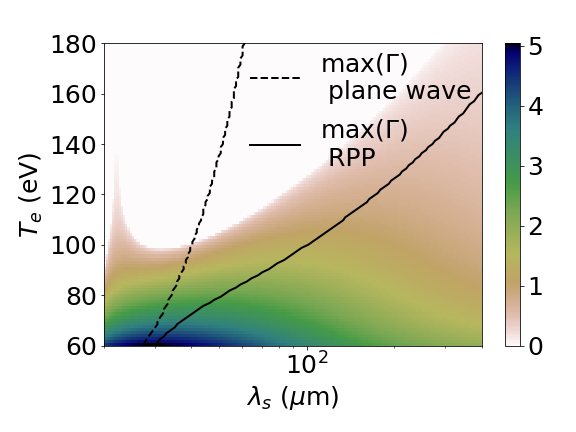
\includegraphics[width=0.24\textwidth]{XpFuchs.png}& 
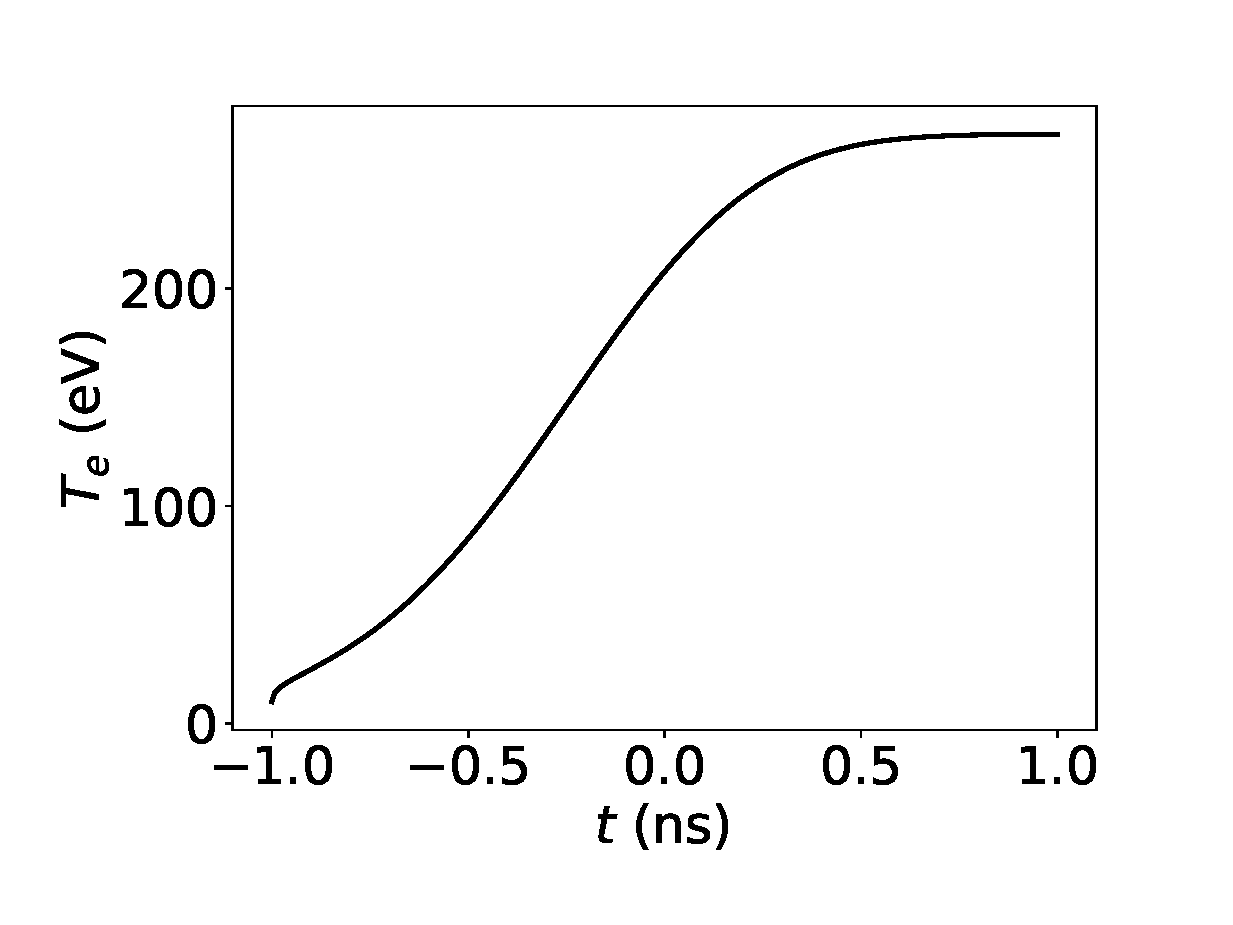
\includegraphics[width=0.24\textwidth]{XpFuchs_te.eps}
\end{tabular}
(c) Experimental RCF \\
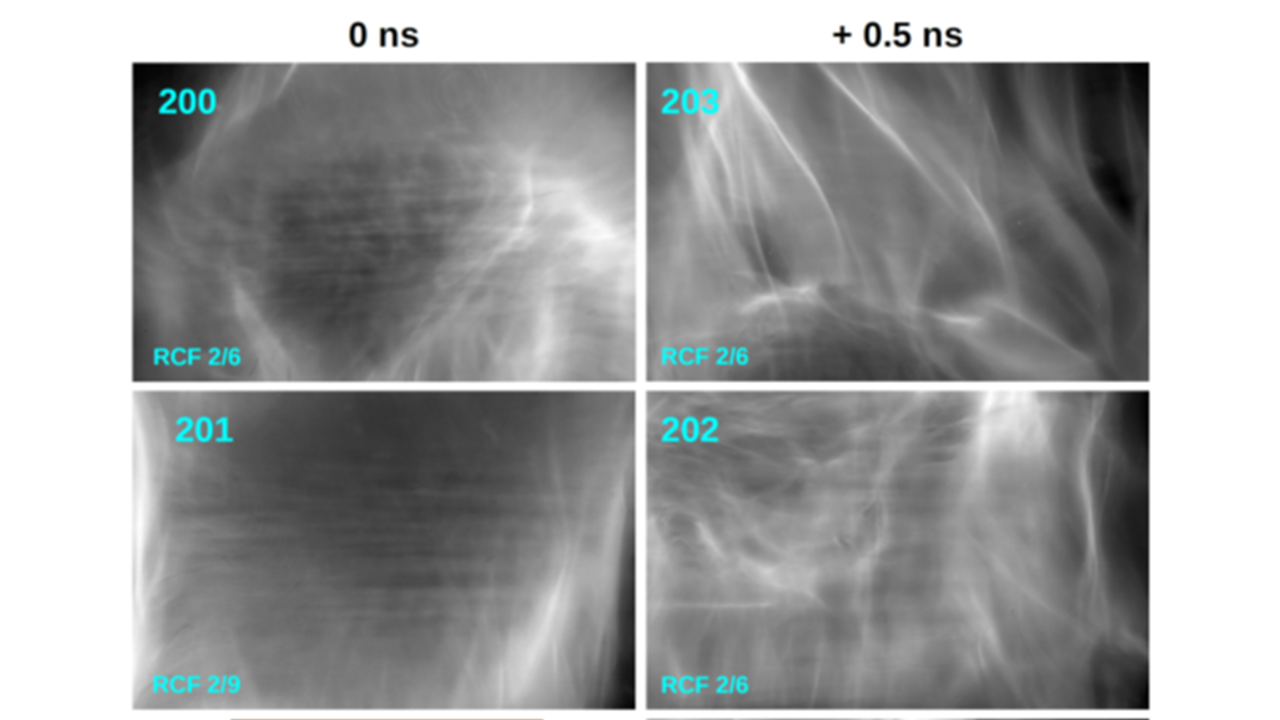
\includegraphics[width=0.5\textwidth]{rcf.png}
\caption{ \label{fig:xpfuchs}  
(a) Solution of Eq. \eqref{eq:dispe2polyrpp} normalized to the plasma length  $L$  for $v_\phi=0$ and in the fluid framework [Eq. \eqref{eq:alphaf}] with $I_0=3.8\times 10^{13}\, \rm W/cm^2$, $2\pi/k_0=1\,\rm\mu m$, $f_\sharp=11$, $Z_i=2$, $A=4$, $n_e=10^{19} \,\rm cm^{-3}$,  $L=1\,\rm mm$ and  $Z_iT_e/T_i=10$. 
The growth rate maximum is superimposed as a  black line in the RPP case and as a dashed line in the plane wave case [Eq. \eqref{eq:dispe2poly}].
(b) Temporal evolution of the electron temperature from an Hydrodynamic simulation  \textcolor{red}{with the code HERA} and from the resolution of $(3/2)n_e d_tT_e=\nu_BI_0\exp(-t^2/\tau^2)/c$ with $\tau = 416\,\rm ps$  and $T_e(-1 \, \rm{ns})=10\,\rm eV$ (black line).
(c) Experimental RCF from four shots of the LULI experiment, at $0$ and $0.5$ ns after the maximum intensity reaching \textcolor{red}{the center of the plasma slab}. 
 }
\end{figure}
\textcolor{red}{Section non finalis\'ee, \'a l'\'etat de note pour plus tard. Il faut une simulation HERA en accord avec l'XP. Mais j'ai l'impression que meme purement analytiquement c'est interessant.}

A low temperature plasma may also be filamentation-unstable to the  propagation of an RPP pulse.
For a single ion species plasma, and provided $ZT_e\gg T_i$,   we recall that $\alpha_f(0)=1\simeq \alpha_k(0)$, for this reason, the filamentation growth con\"incides in both  kinetic and hydrodynamic frameworks. 
Hence, restricting, in this section, the analysis to the fluid plasma response, we aim at comparing our predictions with the filamentation observed at relatively low temperature resulting from a numerical simulation and measured by mean of the proton-radiographic techniques of RPP pulse propagating  in a helium gaz jet.

The colormap of Fig. \ref{fig:xpfuchs}(a) illustrates the RPP filamentation spatial  growth normalized to the plasma length ($L=1\,\rm mm$) as a function of the wavelength and of the electron temperature for the experimental parameters, $I_0=3.8\times 10^{13}\, \rm W/cm^2$, $2\pi/k_0=1\,\rm\mu m$, $f_\sharp=11$, $Z_i=2$, $A=4$ and $n_e=10^{19} \,\rm cm^{-3}$. Moreover, the choice has been made to fix the ratio  $Z_iT_e/T_i=10$, and the laser is modeled by a Gaussian of $500\,\rm ps$ FWHM and maximum intensity $I_0=3.8\times 10^{13}\, \rm W/cm^2$. The RPP growth rate maximum (black plain line) demonstrates that a reasonable gain is obtained,  $G=\Gamma L\gtrsim 3-5$, when $T_e\lesssim 80\, \rm eV$, \emph{i.e} roughly half a nanosecond before the pulse maximum intensity  [see Fig. \ref{fig:xpfuchs}(b)]. 
This suggests that the filamentation grows and saturates rapidly before the most energetic part of the beam reaches the center of the gaz jet, leading to  density fluctuations of wavelength   $\lambda_F \simeq 80-100 \,\rm\mu m$. The resulting electrostatic field is able to deflect the probing protons, which, once collected on a stack of radiochromic films, causes the proton dose modulations illustrated in Fig \ref{fig:xpfuchs}(c). Averaging the distance between the filamentary structures, we obtain an estimated experimental wavelength of $\simeq 84 \,\rm\mu m$ in very good accordance with our RPP dispersion relations. 
Note that the textbook plane wave filamentation dispersion relations [Eq. \eqref{eq:dispe2poly} for $v_\phi=0$] predicts a much smaller dominant wavelength of $20\, \rm{\mu m} \lesssim \lambda_F\lesssim  35\, \rm\mu m$ (when $70\, \rm{eV}<T_e<140\, \rm eV$), illustrated as a dashed black line in Fig. \ref{fig:xpfuchs}(a) thus demonstrating the significance of our random phase plates dispersion relations regarding realistic conditions. 


\subsection{Forward Brillouin scattering of a  spatially smoothed beam}
Figures \ref{fig:disperpp} and \ref{fig:dispeCHrpp} shows also significant differences compared to the propagation of a plane wave  regarding the forward Brillouin scattering.  
Either Fluid or kinetic, for single or multiple ion species, 
the spatial growth rate appears much more peaked around $v_\phi\simeq c_s$ [or $v_\phi\simeq 0.8c_s$ for  the kinetic CH case, Fig. \ref{fig:dispeCHrpp}(a)] and the propagation of the RPP pulse more unstable  [$\Gamma/k_0\sim 0.01$, Fig.  \ref{fig:disperpp}(a) and $\Gamma/k_0\sim 0.05$, Fig.  \ref{fig:dispeCHrpp}(a)]  than for a plane wave case  [$\Gamma/k_0\simeq 2 \times 10^{-4}$, Fig.  \ref{fig:dispe}(a)].
Therefore degrading the pump spatial coherence does subjugate the filamentation instability (or at least significantly reduces it for the CH-case), however, at the expense of favoring the Brillouin instability.
The forward scattering of an RPP beam ensues from the superposition of all the pulse spectral contributions, the final superposition of acoustic waves may be constructive or destructive depending on the wavevector direction and amplitude. As a consequence, the spatial growth consists in a succession of peaks aligned around $v_\phi\simeq c_s$ and spread from $\vert k_s\vert=0$ to a fraction of $k_0$. The separation of these peaks [a few $ 10^{-2}k_0$ for Fig. \ref{fig:disperpp}(a) and $\sim 10^{-1}k_0$ for \ref{fig:dispeCHrpp}(a)], depends on the propagation properties of the driven acoustic waves such as the effective damping rate and the wavevector direction. 
The factor $\alpha_{k/f}$ [Eqs. \eqref{eq:alphak} and  \eqref{eq:alphaf}] that  holds the acoustic waves propagation characteristics, contrasts  in the fluid and in the kinetic framework for $\vert v_\phi\vert>0$ and $Z_iT_e/T_i\lesssim 10$ thus explaining the disparities between Figs. \ref{fig:disperpp}(a) and (c) [as well as  \ref{fig:dispeCHrpp}(a) and (c)], such as the spectral distribution of the unstable clusters. 
Figures \ref{fig:disperpp}(a,c) presents twice more unstable peaks in the fluid (c) than in the kinetic (a) framework, and apart from that,  surprisingly similar growth behavior are obtained, either in the single or multi ion species case. 

Regarding the propagation of an RPP pulse, the growth spectral width has to be compared with the  beam width in vacuum $k_m/k_0=1/(2f_\sharp)$. 
For the H$^+$-plasma, 
the range  $0.05 \lesssim k/k_0\lesssim 0.2$ 
is unstable thus probably 
leading to the increase of the $f_\sharp$-cone 
angle from $1/(2f_\sharp)=3.6^o$ to $11.5^o$. 
Hence, a large modification of beam 
propagation properties  should appear during its propagation thus affecting the energy deposition outcomes.
Regarding the CH-plasma, one may notice that unlike for the single ion case, the peaks are located around $v_\phi=0.8c_s$, implying a lower acoustic frequency (than for the single ion species case or than the fluid calculations) and thus less red-shifting of the scattered wave.
Two and four unstable peaks are evidenced in Figs. \ref{fig:dispeCHrpp}(a) and (c), corresponding to $\sim (9^o,14^o)$ and $ \sim (6.5^o,8.5^o,11.5^o,15^o)$ scattering direction, respectively.
Albeit  a similar growth rate  predicted by the kinetic and fluid calculations, different scattering directions are obtained which indicates that the fluid framework  suffers, in some cases, from an ill-forecast of the beam spectral properties. 

\textcolor{red}{Comparison with dedicated PIC simulation in periodic geometry}


\section{Conclusion}
The spatial growth of the  pump wave filamentation and of the forward Brillouin instabilties, as derived in this study, enables the comparison of both instabilities in the fluid and kinetic frameworks. They confirm the importance  of spatial smoothing techniques on the control of the laser filamentation and pinpoints that, in some cases such as multi-ion  or cold-enough  plasmas, this instability may survive.
Moreover, we also conclude that the use of Random phase plates may further destabilize the laser propagation   regarding FSBS,  leading to larger angle scattering and thus stronger modification of the energy deposition.
Provided one accounts for multi-ion species and non-local thermal corrections, working in the fluid framework seems to be reasonable regarding the laser filamentation. 
Albeit similarities between the hydrodynamic and kinetic model, the forward Brillouin scattering of an RPP pulse also brings to light the significance of    driven acoustic  wave damping able to  affect  the predicted  scattering spectrum.

The use of SSD, which  causes the so-called speckles to vanish and change position, is known  experimentally to significantly stabilize the pump propagation. The framework developed in this publication  allows the insertion of spectral dispersion in the dispersion relations of importance for LMJ or NIF like facilities  and is left for future work. Moreover, 
combining the results of  Ref. \cite[]{POP_Debayle_2019} with our spatial growth rates opens the way for 
including the RPP forward Brillouin scattering   in the vastly used ray tracing schemes, possibly greatly improving their prediction precision regarding high-energy laser experiments.
Finally, the comparison of our model with NIF or LMJ-relevant experiments is currently underway. 

%\textcolor{red}{
%Todo
%\begin{itemize}
%    \item PRL Sarri 2011
%    \item Nat phys. 3 Glenzer 2007 p716
%    \item Lushnikov 2006
%    \item ...
%\end{itemize}
%}

\section*{Acknowledgements}
We acknowledge important discussions with M. Grech and also admit the role of the confinement following the COVID19 plague for forcing us to take the time to finalize this theoretical work. This work has been done under the auspices of CEA-DAM. 
% and the simulations were performed using HPC resources at TGCC/CCRT and CEA-DAM/TERA.
\bibliography{biblio}
\end{document}
